\usepackage[authoryear,round]{natbib}
\usepackage{multirow}

\newcommand{\sheetnum}{%
	03
}
%\setcounter{section}{\sheetnum-3}
\newcommand{\tutorialtitle}{%
    Kernel Principal Component Analysis
}
\newcommand{\tutorialtitleshort}{%
	Kernel PCA (non-linear PCA)
}
% for slides
\subtitle{\sheetnum \tutorialtitle}

\maxdeadcycles=1000 % Workaround for ! Output loop---100 consecutive dead cycles because of too many figures

% The following use of algroithms is recommended for the notes:
%
%\begin{figure}[!t]
%\removelatexerror
%\begin{algorithm}[H]
    % your algo here
    %\label{alg:algolabel}
    %\caption{algocaption}
%\end{algorithm}
%\end{figure}
%\begin{algorithm}
% Below is the definition for the command \removelatexerror:
\makeatletter
\newcommand{\removelatexerror}{\let\@latex@error\@gobble}
\makeatother

\begin{document} %%%%%%%%%%%%%%%%%%%%%%%%%%%%%%%%%%%%%%%%%%%%%%%%%%%%%%%

\sheet{\sheetnum}{\tutorialtitleshort}

\ttopic{\tutorialtitle}

\begin{frame}
\titlepage
\end{frame}

\begin{frame}
\setcounter{tocdepth}{2}
\tableofcontents
\end{frame}

\newpage

% The variable mycolumnleft is set in the minotes class
% The column settings are ignored by the slides
\columnratio{\mycolumnleft,1-\mycolumnleft}
\begin{paracol}{2}
%\setlength{\columnseprule}{0.1pt}
%\setlength{\columnsep}{5em}

\begin{rightcolumn}

\mode<all>

\section{linear PCA: Recap}

\begin{frame}\frametitle{\secname}
\begin{itemize}
\item Requires \pause

 centering the data.
\only<2>{
\slidesonly{
\begin{center}
	\includegraphics[width=0.3\textwidth]{img/mem_notthisagain}%
\end{center}
}
}

\pause
 
\item Eigenvalue problem: $\vec C\,\vec e = \lambda \vec e$
\item limited to \underline{linear} correlations
\end{itemize}


\begin{center}
	\includegraphics[width=0.5\textwidth]{img/scatter}%
	\captionof{figure}{linear vs. non-linear correlations}
\end{center}

Kernel PCA for finding non-linear features.\\


\end{frame}

\begin{frame}\frametitle{What is Kernel PCA about?}

Don't panic! Kernel PCA is essentially standard linear PCA applied to a non-linearly transformed version of the data.

\begin{center}
	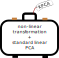
\includegraphics[width=0.3\textwidth]{img/koffer}%
\end{center}

\end{frame}

\mode*

\clearpage


\mode<all>

\section{Non-linear transformations}

We use $N$ to denote the dimensionality of our input space and $p$ to denote the number of observations.\\
Let $\vec x^{(\alpha)} \in \R^N$ and $\alpha = 1, \ldots, p$.

The following mapping describes the non-linear transformation of each observation:
$$
\vec{\phi}: \vec{x} \mapsto \vec{\phi}_{(\vec{x})}
$$

An example of such a transformation - 2\textsuperscript{nd}-order monomials:
$$
\vec{\phi}_{(\vec{x})} = ( 
    1, \;
    \mathrm{x}_1, \;
    \mathrm{x}_2, \;
    \ldots \;
    \mathrm{x}_N, \;
    \mathrm{x}_1^2, \; 
    \mathrm{x}_1 \mathrm{x}_2, \;
    \mathrm{x}_2^2, \;
    \mathrm{x}_1 \mathrm{x}_3, \;
    \mathrm{x}_2 \mathrm{x}_3, \;
    \mathrm{x}_3^2, \; \ldots, \;
    \mathrm{x}_N^2
    )^\top
$$

We actually don't need to define this transformation.
All we need to know is that the dimensionality of $\vec{\phi}_{(\vec{x})}$ can be larger than $N$, possibly infinitely large.\\

\underline{The purpose of non-linear transformations:}

Two or more components in the original $\vec x$ (e.g. $x_1$, $x_2$) could have non-linear correlations (e.g. plotting those two components reveals a parabola). 
Expanding the dimensionality of $\vec x$ through the above mapping introduces new dimensions in which correlations between the components in $\vec \phi_{(\vec x)}$ become \emph{linear}.

\textbf{Caveat}:\\
Directly applying this transformation on a single observation is not applicable. 
We might never find a transformation that causes all non-linear correlations within $\vec x$ to become linear.

We turn to the ``kernel trick'' to solve this problem.

\mode*

\clearpage


\mode<all>
\section{The kernel trick}

\begin{frame}\frametitle{\secname}

Representing a non-linear transformation using inner products of the data:
\begin{equation}
 \label{eq:trick}
      \vec{\phi}_{(\vec{x})}^\top 
		\vec{\phi}_{(\vec{x}')} = 
      k(\vec{x}, \vec{x}')
\end{equation}
    
where $k(\vec{x}, \vec{x}')$ is a kernel function applied 
to any two observations.

\end{frame}

\subsection{The Kernel matrix}

\begin{frame}\frametitle{\subsecname}

Applying the kernel function to \emph{each} pair in our dataset; \\
$\vec x^{(\alpha)}$ and $\vec{x}^{(\beta)}$ 
with $\alpha, \beta = 1, \ldots, p$ yields the scalar $K_{\alpha \beta}$. 
Storing all scalars $K_{\alpha \beta} \; \forall (\alpha,\beta)$ yields 
the un-normalized kernel matrix $\widetilde {\vec K}=\{K_{\alpha \beta}\}$:

\begin{equation}
\widetilde {\vec K} = 
\rmat{
K_{11} & K_{12} & \ldots & K_{1p} \\
K_{21} & K_{12} & \ldots & K_{2p} \\
\vdots & & \ddots\\
K_{p1} & & & K_{pp}
}
\end{equation}

$\vec K$ (without the ``\textasciitilde'') denotes the normalized or ``centered'' kernel matrix. \notesonly{cf. \sectionref{sec:centerkernel} why and how to center the Kernel matrix.}

\question{What is the dimensionality of $\widetilde {\vec K}$?}

\end{frame}

\subsubsection{Properties of the Kernel matrix}

\begin{frame}\frametitle{\subsubsecname}

\begin{block}{From Mercer's theorem}
Every positive semidefinite kernel k corresponds to a scalar product in
some metric feature space.
\end{block}

\end{frame}

\begin{frame}\frametitle{The RBF Kernel}

The Radial Basis function (RBF) 

\question{Is $K_{\alpha \beta}$ sensitive to translation and rotation of the data?}

- No. $K_{\alpha \beta}$ is the pairwise relation between two observations. 
Rotating the data or translating it will result in the same $K_{\alpha \beta}$. 
However, scaling the data while keeping the kernel function fixed would produce a different $K_{\alpha \beta}$.

\end{frame}

\mode*

\clearpage

\mode<all>

\section{Kernel PCA}

We apply standard linear PCA on the \emph{transformed} version of the data
$
\left\{
\vec{\phi}_{(\vec{x}^{(\alpha)})}
\right\}_{\alpha=1}^{p}
$.
We will first assume we have $\vec{\phi}_{(\vec{x})}$ 
but we will eventually turn to $K_{\alpha \beta}$ 
which we can actually obtain.\\

\underline{Remark:}
A difference between these notes and the lecture slides is that 
the lecture slides employ ``identity'' as the mapping. 
This is why you don't see $\phi$ in the derivations of Kernel PCA in the slides but rather see $\vec x$ used directly.\\

\begin{enumerate}
\item PCA assumes its input is centered. 
$\frac{1}{p} \sum^{p}_{\alpha=1} \vec{\phi}_{(\vec{x}^{(\alpha)})}$\\
Centering $\vec X$ does not guranatee it stays centered after transformation.
Therefore, there is no need to center $\vec X$ beforehand.

\item Compute the covariance matrix $\vec C_{\phi}$ for $\vec{\phi}_{(\vec{x})}$:


\begin{equation} \label{eq:cov}
\vec C_{\phi} = \frac{1}{p} \sum_{\alpha=1}^{p} \vec{\phi}_{(\vec{x}^{(\alpha)})} \vec{\phi}^{\top}_{(\vec{x}^{(\alpha)})}
\end{equation}

\item Solve the eigenvalue problem:

\begin{equation} \label{eq:eig}
\vec C_{\phi} \, \vec e = \lambda \vec e
\end{equation}

Each eigenvector $\vec e_i$ with corresponding $\lambda_i \ne 0$ lies in the span of 
$
\left\{
\vec{\phi}_{(\vec{x}^{(\alpha)})}
\right\}_{\alpha=1}^{p}.
$

Consequently, there exists a set of coefficients (i.e. a coefficient for each transformed observation)
$
\left\{
a^{(\alpha)}
\right\}_{\alpha=1}^{p}
$, which satisfies the following:

\begin{equation}
\label{eq:ephi}
\vec e = \sum^{p}_{\beta=1} a^{(\beta)} \vec{\phi}_{(\vec{x}^{(\beta)})}
\end{equation}

Eq.\ref{eq:ephi} tells us that we can describe $\vec e$ in terms of the transformed observations (a weighted summation of $\phi$'s).
 The use of the index $\beta$ is only to avoid collisions with $\alpha$ later.

Substituting Eq.\ref{eq:cov} and Eq.\ref{eq:ephi} into the eignevalue problem Eq.\ref{eq:eig}:

\begin{equation*}
\underbrace{\frac{1}{p} \sum_{\alpha=1}^{p} \vec{\phi}_{(\vec{x}^{(\alpha)})} \vec{\phi}^{\top}_{(\vec{x}^{(\alpha)})} 
}_{=\,\vec C_{\phi}}
 \, 
\underbrace{\sum^{p}_{\beta=1} a^{(\beta)} \vec{\phi}_{(\vec{x}^{(\beta)})}}_{=\,\vec e}
 = \lambda \;\,
\underbrace{\sum^{p}_{\beta=1} a^{(\beta)} \vec{\phi}_{(\vec{x}^{(\beta)})}}_{=\,\vec e}
\end{equation*}

After rearranging the terms we get:
\begin{equation} \label{eq:eig2}
\frac{1}{p} \sum_{\alpha=1}^{p} \sum^{p}_{\beta=1} 
a^{(\beta)} \vec{\phi}_{(\vec{x}^{(\alpha)})}
\underbrace{
 \vec{\phi}^{\top}_{(\vec{x}^{(\alpha)})} \,  \vec{\phi}_{(\vec{x}^{(\beta)})}
}_{\substack{\text{scalar product}\\ = K_{\alpha\beta}}}
 = \lambda 
\sum^{p}_{\beta=1} a^{(\beta)} \vec{\phi}_{(\vec{x}^{(\beta)})}
\end{equation}

Recall that we cannot compute $\vec{\phi}_{(\vec{x})}$ but can now 
exploit the kernel trick (cf. Eq.\ref{eq:trick}) by substituing 
$ K_{\alpha \beta} $ for
$
\vec{\phi}^{\top}_{(\vec{x}^{(\alpha)})}
 \, 
  \vec{\phi}_{(\vec{x}^{(\beta)})}
$

Eq.\ref{eq:eig2} becomes:
\begin{equation} \label{eq:eig3}
\frac{1}{p} \sum_{\alpha=1}^{p} \sum^{p}_{\beta=1} 
a^{(\beta)}
\vec{\phi}_{(\vec{x}^{(\alpha)})} K_{\alpha \beta}
 = \lambda 
\sum^{p}_{\beta=1} a^{(\beta)} \vec{\phi}_{(\vec{x}^{(\beta)})}
\end{equation}

We will now proceed with reformulating the above until we no longer have any $\phi$'s.

We left-multiply Eq.\ref{eq:eig3} with $\left(\vec \phi^{(\gamma)}\right)^\top$, where $\gamma = 1, \ldots, p$.
 We can pull $\left(\vec \phi^{(\gamma)}\right)^\top$ directly into the sum on the left and the sum on the right:

\begin{equation} \label{eq:eig4}
\frac{1}{p} \sum_{\alpha=1}^{p} \sum^{p}_{\beta=1} 
a^{(\beta)}
\underbrace{
\left(\vec \phi^{(\gamma)}\right)^\top
\vec{\phi}_{(\vec{x}^{(\alpha)})} 
}_{=K_{\gamma \alpha}}
K_{\alpha \beta}
 = \lambda 
\sum^{p}_{\beta=1} a^{(\beta)} 
\underbrace{
\left(\vec \phi^{(\gamma)}\right)^\top \vec{\phi}_{(\vec{x}^{(\beta)})}
}_{=K_{\gamma \beta}}
\end{equation}

\newpage

Eq.\ref{eq:eig4} without the clutter:

\begin{equation} \label{eq:eigK}
\frac{1}{p} \sum_{\alpha=1}^{p} \sum^{p}_{\beta=1} 
a^{(\beta)}
K_{\gamma \alpha}
K_{\alpha \beta}
 = \lambda 
\sum^{p}_{\beta=1} a^{(\beta)} 
K_{\gamma \beta} \quad \forall \gamma
\end{equation}

Since we want to compute this for all training samples $\gamma$, 
we can reduce the clutter even more by using matrix notation. 
Specifically, by using the \emph{kernel matrix} $\vec K=\{K_{\alpha\beta}\}$, where \\
$
K_{\alpha \beta} = 
k(\vec x^{(\alpha)}, \vec x^{(\beta)}) = 
\vec{\phi}_{(\vec{x}^{(\alpha)})}^\top 
		\vec{\phi}_{(\vec{x}^{(\beta)})}
$ 

We end up with this formulation of the eigenvalue problem:

\begin{equation*}
	\vec{K}^2 \vec{a} = p \lambda \vec{K} \mspace{2mu} \vec{a}
\end{equation*}

$\vec K$ appears on both sides. All the solutions that are of interest remain represented in 
the following simpler eigenvalue problem, which we refer to as the \emph{transformed eigenvalue problem}:
\begin{equation}
\label{eq:eigsimple1}
	\vec{K} \, \vec{a} = p \lambda \mspace{2mu} \vec{a}
\end{equation}

We can interpret $\vec a$ as the \emph{eigenvector} of $\vec K$

By omitting the constant $p$, we can rely on finding solutions for $\lambda$ that absorb it:

\begin{equation}
\label{eq:eigsimple2}
	\vec{K} \, \vec{a} = \lambda \mspace{2mu} \vec{a}
\end{equation}

All we've been doing so far is reformulate the eigenvalue problem such that we end up 
with a formulation that only contains terms of the inner product kernel.\\
Why was all this necesary? Because (1) we want to enable PCA to find non-linear correlations and (2) we don't have access to $\vec \phi_{(\vec x)}$.

Now that we've solved the eigenvalue problem, we continue with the remaining steps for PCA.

\newpage 
\item Normalize the eigenvectors:

Before we can project anything onto the space spanned by the PCs $\widetilde{\vec a}_k$ where $k=1,\ldots,p$,
we need to ensure these vectors are normalized. 
$\widetilde {\vec a}_k$ is only used to indicate that the vector has not been normalized yet.

%$\widetilde {\vec a}_k$ can be normalized explicitly by:
%$$
%\vec a_k^{norm.} = \frac{1}{||\widetilde{\vec a}_k||} \cdot \widetilde{\vec a}_k = 
%\frac{1}{\sqrt{\left(\widetilde{\vec a}_k\right)^\top \widetilde{\vec a}_k}} \cdot \widetilde{\vec a}_k
%$$

%However, we want to demonstrate how to normalize $\widetilde {\vec a}_k$ in a way that can be more efficient than an explicit normalization.

Recalling Eq.\ref{eq:ephi} (we add the index $k$ to denote which eigenvector):
\begin{equation}
\label{eq:ephik}
\vec e_k = \sum^{p}_{\beta=1} a_k^{(\beta)} \vec{\phi}_{(\vec{x}^{(\beta)})},
\end{equation}

Again, we try to reformulate things such that we end up with the inner-product kernel rather than $\phi$. 
We left-multiply Eq.\ref{eq:ephik} with $\left(\vec e_k\right)^\top$:
\begin{align}
\vec e^{\top}_k \vec e_k &= \sum^{p}_{\alpha=1}  a_k^{(\alpha)} \vec{\phi}_{(\vec{x}^{(\alpha)})}^\top \sum^{p}_{\beta=1} a_k^{(\beta)} \vec{\phi}_{(\vec{x}^{(\beta)})} \\
&= \sum^{p}_{\alpha=1}  \sum^{p}_{\beta=1}  a_k^{(\beta)}  \underbrace{\vec{\phi}_{(\vec{x}^{(\alpha)})}^\top  \vec{\phi}_{(\vec{x}^{(\beta)})}} a_k^{(\alpha)} \\
&= \sum^{p}_{\alpha=1}  \sum^{p}_{\beta=1}  a_k^{(\beta)} \quad \; K_{\alpha\beta} \quad \; a_k^{(\alpha)} \\
&= \widetilde {\vec a}_k^\top \vec K \, \widetilde {\vec a}_k
\end{align}

And when we plug Eq.\ref{eq:eigsimple1} into the above:

\begin{equation}
\label{eq:eignorm}
\vec e^{\top}_k \vec e_k = 
\widetilde {\vec a}_k^\top 
\underbrace{p \lambda_k \, \widetilde {\vec a}_k}_{=\, \vec K \, \widetilde {\vec a}_k} 
= p \lambda_k \, \widetilde {\vec a}_k^\top \widetilde {\vec a}_k  \eqexcl 1
\end{equation}

Scaling $\widetilde {\vec a}_k$ by $\frac{1}{\sqrt{p \lambda_k}}$ yields 
a unit vector with the same direction as $\widetilde {\vec a}_k$ to satisfy Eq.\ref{eq:eignorm}.\\
With
\begin{equation}
\vec a_k^{norm.} := \frac{1}{\sqrt{p \lambda_k}} \widetilde {\vec a}_k,
\end{equation}
follows:
\begin{align}
\vec e^{\top}_k \vec e_k 
&= p \lambda_k \, \; \widetilde {\vec a}_k^\top \; \widetilde {\vec a}_k\\
&= p \lambda_k \, \left(\vec a_k^{\text{norm.}}\right)^\top \vec a_k^{\text{norm.}} \\
&= p \lambda_k \left(\frac{1}{\sqrt{p \lambda_k}} \widetilde {\vec a}_k\right)^\top \left(\frac{1}{\sqrt{p \lambda_k}} \widetilde {\vec a}_k\right)
= 1
\end{align}


\newpage

\item Sort the eigenvectors such that the corresponding eigenvalues are arranged in decreasing order. 


\item Projection:

In order to project some observation $\vec x$ into the PC space, we first map it into the non-linear space of $\phi$ 
and then project that into the space spanned by the PCs. 
By now we should expect that the transformation can only be performed via the kernel trick. 
We basically represent this sample $\vec x$ by its relation to the \emph{training data} 
(i.e. the $p$ observations that were used to compute the PCs).

We derive the projection for Kernel PCA by starting with the projection used in linear PCA (cf. slides 1.3 \#11):

The projection for linear PCA, specifically the component of $\vec x$ in the direction of the $k$-th PC is:
\begin{equation}
\label{eq:projlin}
u_k(\vec x) = \vec e_k^\top \vec x
\end{equation}

We substitute $\vec \phi_{(\vec x)}$ for $\vec x$ and plug Eq.\ref{eq:ephi} into Eq.\ref{eq:projlin}:

\begin{align}
\label{eq:projk1}
u_k(\vec \phi_{(\vec x)}) &= \sum^{p}_{\beta=1} a^{(\beta)} 
\underbrace{
\vec{\phi}^\top_{(\vec{x}^{(\beta)})} \vec \phi_{(\vec x)}
}_{\substack{
\text{recognize the familiar}\\
\text{scalar product?}
\\ =k(\vec x^{(\beta)}, \vec x) = K_{\beta,\vec x}}}\\
&= \sum_{\beta=1}^{p} a_k^{(\beta)} K_{\beta, \vec x}
\end{align}

Note that $\vec x$ can be a sample that was used in computing the PCs or a completly new ``test'' point.

\item Reconstruction:

Since we never had the transformation $\phi$ to begin with. 
It is not psssible to simply project a sample from PC space back into the original $N$-dimensional input space. 
Algorithms exist that approximate a ``pre-image'' of some new observation.
\end{enumerate}

\mode*

\clearpage

\mode<all>
\subsection{Centering the kernel matrix}

\label{sec:centerkernel}

\begin{frame}{\subsecname}

PCA operates on centered data. This is common for all forms  of PCA, 
whether it is linear PCA, online PCA or Kernel PCA.\\
In Kernel PCA, the $\vec X$ is transformed into a higher dimensional space by applying the kernel trick.
Applying it to all $p$ training samples yields the kernel matrix, which is used in solving the transformed eigenvalue problem.

All of the above assumed that we have successfully centered the kernel matrix. We now look at how this is done.

\end{frame}


\begin{frame}{\subsecname}


\question{Do I need to center $\vec X$ before computing $ K_{\alpha \beta}$?}

\pause

- No, Centering $\vec X$ before computing $K_{\alpha \beta}$ does not guarantee the kernel matrix to be centered. You only end up with $\vec{\widetilde K}$. The same applies if we had the $\phi$'s.

It is simply irrelevant whether the original data $\vec X$ is centered or not. 
Therefore, we need to center the kernel matrix before solving the transformed eigenvalue problem.\\

\end{frame}

\begin{frame}{\subsecname}

\notesonly{
We use $\vec{\widetilde K}$ to denote the \emph{un-normalized} kernel matrix and $\vec K$ 
to denote the kernel matrix \emph{after} it has been centered.\\
}

%\underline{Centering $\vec{\widetilde K}$:}

The centering is built on the kernel trick\notesonly{ as in Eq.\ref{eq:trick}}:
\begin{equation}
      k(\vec{x}, \vec{x}') = K_{\vec x,\vec x'} = \vec{\phi}_{(\vec{x})}^\top 
		\vec{\phi}_{(\vec{x}')},
\end{equation}

except that we compute the inner product using \emph{centered} $\phi_{(\vec x)}$:

\begin{equation}
	\underbrace{ \vec{\phi}_{\big( \vec{x}^{(\alpha)} \big)} }_{
		\substack{ 	\text{centered} \\
				\text{feature vectors}} }
				\hspace{-3mm}
	= \widetilde{\vec{\phi}}_{\big( \vec{x}^{(\alpha)} \big)}
				\hspace{-1mm}
		- \frac{1}{p} \sum\limits_{\gamma = 1}^p 
				\hspace{-2mm}
		\underbrace{ \widetilde{\vec{\phi}}_{\big( \vec{x}^{(\gamma)} 
				\big)} }_{
			\substack{ 	\text{uncentered} \\
					\text{feature vectors}} }
					\qquad \forall \alpha
\end{equation}

\notesonly{
Plugging \emph{centered} $\vec{\phi}_{(\vec{x})}$ into the kernel trick equation\slidesonly{ above} reveals how to obtain centered elements $K_{\alpha\beta}$ for }forming a \emph{centered} \notesonly{Kernel matrix }$\vec K$ from an \emph{unnormalized} \notesonly{Kernel matrix }$\widetilde{\vec K}$.

\begin{equation}
	K_{\alpha \beta} = \underbrace{\widetilde{K}_{\alpha \beta}}_{ _{= \, k \left ( \vec{x}^{(\alpha)},
			\vec{x}^{(\beta)} \right )}}
		- \;\underbrace{\frac{1}{p} \sum\limits_{\delta = 1}^p 
		\widetilde{K}_{\alpha \delta}}_\text{\scriptsize{row avg.}} 
		\; - \; \underbrace{\frac{1}{p} 
		\sum\limits_{\gamma = 1}^p 
		\widetilde{K}_{\gamma \beta}}_\text{\scriptsize{col. avg.}}
		\;+ \;\underbrace{\frac{1}{p^2} 
		\sum\limits_{\gamma, \delta = 1}^p 
		\widetilde{K}_{\gamma \delta}}_\text{\scriptsize{matrix avg.}}
\end{equation}%


\end{frame}


\mode*

\clearpage

\mode<all>


\subsection{Applying Kernel PCA}

\begin{frame}{How do I interpret the role of PCs?}

\notesonly{\question{How do I interpret the role of PCs?}}

\svspace{-7mm}

\begin{center}
	\includegraphics[height=5cm]{img/contourplot_kpca_rbf}
	\notesonly{\captionof{figure}{Projections onto individual PCs}}
\end{center}
\svspace{-0.8cm}
\begin{center}
	\includegraphics[height=3.2cm]{img/screeplot_kpca_rbf.pdf}
	\notesonly{\captionof{figure}{Scree plot}}
\end{center}

\end{frame}

\subsection{A note on implementation}

\begin{frame}{\subsecname}

\question{Should you solve the transformed eigenvalue problem using \emph{eigenvalue decomposition} or \emph{SVD}?}

\slidesonly{
\begin{equation}
%\label{eq:eigsimple1}
	\vec{K} \, \vec{a} = p \lambda \vec{a}
\end{equation}
}

\pause

- \emph{eigenvalue decomposition} is the only option for Kernel PCA. \emph{SVD} is simply not applicable since we don't have access to $\vec \phi_{((\vec x))}$

\begin{equation}
 %\label{eq:cov}
\vec C_{\phi} = \frac{1}{p} \sum_{\alpha=1}^{p} \vec{\phi}_{(\vec{x}^{(\alpha)})} \vec{\phi}^{\top}_{(\vec{x}^{(\alpha)})}
\end{equation}

\end{frame}

\begin{frame}{\subsecname}

\question{Which property of $\widetilde {\vec{K}}$ can we exploit to speed up computation?}

\pause

The kernel function is symmetric. $k(\vec x^{(\alpha)}, \vec x^{(\beta)}) = k(\vec x^{(\beta)}, \vec x^{(\alpha)})$. One can exploit this by reducing how many times the kernel function is actually applied while traversing the training samples when computing $\widetilde {\vec{K}}$.

\end{frame}

%TL;DR: Picking the right parameters for the kernel depends on how good that parameter solves your problem (good dim. reduction, reflects certain assumptions about the data - e.g. expected degree of polynomial). We treat them as hyperparameters, so "tuning" them is usually done through cross-validation than gradient-based optimization.

%The long version. This is actually how I end up with more content for the tutorial notes, not always but every now and then it happens. So thank you for the question:

%Finding good parameters for the kernels depends on the data and the task you are trying to solve.
%This comes across as a very generic answer but let's look at two examples. I will use the RBF Kernel which is parameterized by a single parameter sigma. You an easily extend this to other kernels. It also doesn't matter if we're using this kernel for an unsupervised method (e.g. Kernel PCA) or a supervised one (e.g. SVM - don't feel left out if you don't know what an SVM is - just don't tell anyone - people are so judgmental these days tsts):

%Example A: We want to reduce the dimensionality of some high dimensional data (i.e. compression). We start of with N dimensions (N is large), p points (lots of points). Kernel PCA is going to give us p PCs. We perform Kernel PCA once with sigma = sigma_1 and a second time with sigma = sigma_2.
%How do we know which sigma value to use for dimensionality reduction?

%Suggestion 1: Create a scree plot for the eigenvalues obtained from using sigma_1 and compare it to the scree plot from using sigma_2. The ones that gives you "more variance explained" with the least amount of PCs is an indication that one sigma could be better than the other. A scree plot that shows a lot of variance explained for the first couple of PCs and then suddenly drops for all the rest is an indicator that those PCs are enough for good dimensionality reduction. You'll sometimes run into situations where you don't think the comparison shows a clear winner. Therefore,...

%Suggestion 2: Measure and compare reconstruction error between the two sigmas. It's exactly what we're looking for when doing dimensionality reduction. More intuitive than looking at a scree plot but it involves reconstructing and that involves approximations (c.f. lecture slide 1.4 #23) so there's a drawback.
%Something to keep in mind when using reconstruction error is that for the same sigma you get some value for your reconstruction error when measure it for data that you used in training (i.e. solving the eigenvalue problem) vs. the error value you get when reconstructing test data. This is where cross validation comes in. We're going to talk about cross-validation later in the course when we talk about density estimation. Basically, you want to know how well your model does when you feed it data that it's never seen before. If it does well on training data but badly on unseen data, then you can't really deploy this model. So before deploying it you need to measure this performance (e.g. reconstruction error) on unseen data. This is called cross validation and you can use this to compare how well one sigma does vs another. How well does one sigma do on unseen data vs. the other sigma? The sigma that has better cross validation performance is the one you go with.

%Example B: Using Kernel PCA to preprocess data before feeding it into a classifier:
%You've picked a kernel (e.g. RBF) you're trying different values for the sigma. You do Kernel PCA and project the data onto the PCs. You feed the projections into a classifier to tell you if this is an image of a cat or a dog (TODO: cat vs. dog is boring, replace with something that has more bling). You measure the classifier's performance and you find out it gives the correct answer 80% of the time. Redo the above with another sigma and you get 87%. You can use the classifier's performance as a measure for deciding which sigma to use. It's still Kernel PCA but you're hyperparameter selection is based on something completely different. But it's a well justified criterion for that task that you are trying to solve. Calling a parameter a "hyperparameter" implies that you don't used gradient-based optimization to tune it but rather something like cross-validation. The reason for not using gradient-based optimization could be that you performance measure or cost function w.r.t. to that parameter is not necessarily differntiable or it would make the optimization too complicated from all the free parameters.

%A note on the Neural Network kernel (aka tanh Kernel, aka sigmoid kernel):
%The kernel itself is not a neural network. when people saw the expression tanh( xTx + ) resembled an expression we are used to seeing in neural networks. What value do you pick for and ? Scroll up, the same applies and it depends on the data and the task.

\mode*

\clearpage

%\section{References}
%\begin{frame}[allowframebreaks] \frametitle{References}
	%\scriptsize
	%\bibliographystyle{plainnat}
	%\bibliography{bibliography}
%\end{frame}

\end{rightcolumn}
\end{paracol}

\end{document}
